The User Interface (UI) is one of the most important pieces of \textit{Computron}, as it is responsible for providing players with the primary means of interacting with the game in an efficient and enjoyable way.
The UI presents the user with controls to navigate between scenes and solve puzzles, and it is the main source of text-based information that enables the user to learn and proceed with the game.
An overview of the major components of the UI for the puzzle scene can be seen in Figure \ref{fig:ui_sytem_diagram}.\\


\begin{figure}[!hb]
    \caption{UI System Overview}
    \label{fig:ui_sytem_diagram}
    \centering
    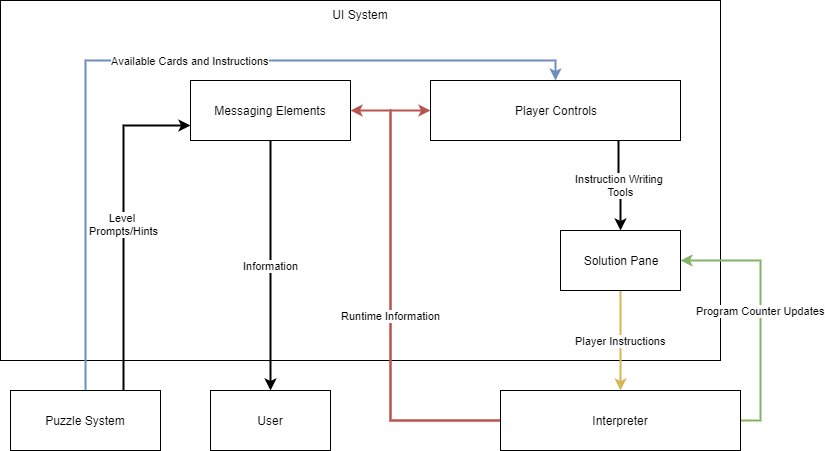
\includegraphics[width=\textwidth]{Diagrams/UI_Overview.png}
\end{figure}


\subsubsection{Information Dissemination}
Controlling the flow of information to the player presented both technical and design
issues to the team. Providing too many hints, prompts, and explanations would quickly
turn the game into a glorified textbook; however, providing too few would make the game
feel frustrating and inaccessible to our target audience. The User Interface was tasked
with providing the right amound of information to the player in an easy to follow sequence.


The UI system communicates with other major game systems to get relevant information, and the UI is responsible for delivering this information to the player at the appropriate times. The data-driven approach of the puzzle system allows it to provide the UI with unique puzzle data for each level of the game. At the start of each level, the UI retrieves from the puzzle system the data that is used to fill out the level's description, prompts, and hints.


\subsubsection{UI Control System}
The puzzle scene contains many UI elements that can be grouped together based on common features, and during development it became clear that certain game states such as tutorialization should trigger similar behaviors (such as focusing, disabling, highlighting, etc.) for entire groups of UI elements at once.
With the significant amount of UI elements in the puzzle scene plus the need for special UI behaviors triggered by the game state, it became necessary to implement a system for giving similar UI elements shared abilities, and to create a centralized means of controlling all UI elements from a single controller.
This need was filled by the UI control system that consists of two primary classes UIController and ControllableUIElement, with multiple subclasses that inherit from ControllableUIElement.


The ControllableUIElement class serves as an interface for the UIControl and UIControlGroup classes.
The UIControl class provides generic UI elements with a few simple methods to bring the object in or out of focus and control whether the object is enabled for the player to use or not.
The UIControlGroup class is used for controllable UI elements that also contain child objects that are also controllable UI elements; it serves as a sort of middle manager. A UIControlGroup can be controlled with the behaviors of a ControllableUIElement, but the UIControlGroup also tracks all of its child objects with a ControllableUIElement component. When a UIControlGroup method is called, the parent group object also has its children run their equivalent method.
Although the generic UIControl class is appropriate for most individual UI objects, there are some special UI elements that need slightly modified behaviors. The CardUIControl, JumpCommandUIControl, and CardCommandUIControl classes inherit from the UIControl class and override the standard methods to fit their special needs.

While all of the ControllableUIElement objects have been granted shared capabilities, they still need to be controlled by a higher power.
The UIController class creates a centralized authority that coordinates and controls all ControllableUIElements.
The UIController finds all ControllableUIElement components and is has many methods to control these UI elements or groups during runtime based on the game state.


% UIController
% ControllableUIElement
% 	UIControl
% 		CardUIControl
% 		JumpCommandUIControl
% 		CardCommandUIControl
% 	UIControlGroup





\subsubsection{Instruction Awarding}
Upon opening a level in the puzzle scene, the puzzle generator tells the user interface which instructions, if any, are being encountered for the first time. Whenever a level is introducing the player to instructions they have not seen before, a sequence of "instruction awarding" is triggered to aid the player. The instruction awarding sequence presents a prominent UI text window that informs the player that new instructions are available, and each new instruction is represented as a "card" object within the instruction awarding window.
The UI Controller brings the instruction awarding panel into focus, while blurring and darkening other portions of the scene.
The player must click on an instruction card to reveal its contents, which includes the name of the new instruction and a description of how it works. Once the player has clicked on every new instruction, they are able to continue with the level.



\subsubsection{Tutorials}
Tutorials are designed to provide novice players with a high level of guidance necessary for them to learn the basics of how to play the game and familiarize them with puzzle mechanics. If a level includes both a tutorial and new instructions, then the tutorial sequence will begin as soon as instruction awarding has been completed. Tutorials provide guidance via a UI text window, and call on the UI Controller to focus and highlight particular UI elements that the player should interact with to complete the tutorial. These tutorials often have multiple steps to complete, so as soon as one step is completed, the UI text changes and the UI Controller focuses on different UI elements that are relevant to the next step. Once the tutorial sequence is complete, the player can continue with normal puzzle gameplay.




\subsubsection{Solution Building and Execution}

A fairly complex custom group of game objects that serves a significant role in the puzzle scene is what we call a "dynamic scroll view".
The puzzle scene contains two instances of dynamic scroll views: the Instruction Cache and the Solution Window. This section will first explain the generic version of the dynamic scroll view and related components, then explain how these components relate to puzzle solution building and execution.


The root object of a dynamic scroll view is a frame that contains a modified scroll view with many more features than a normal Unity scroll view. One of the key features of the dynamic scroll view is the ability for players to add, remove, and reorder its contents during runtime. The dynamic scroll view is meant to contain modified UI buttons with custom code to give the buttons drag and drop behaviors. These drag and drop behaviors allow the player to click and drag the object, move it around with the mouse, then drop it into an object with the Instruction Container script which allows it to catch draggable objects. The special objects with the drag and drop behaviors became the foundation of the UI instruction objects that are used in the Instruction Cache and the Solution Window.


When draggable instruction objects are dragged over a dynamic scroll view, a blank slot spawns in the scroll view content panel as a placeholder for where the button would be placed if it is dropped. If there are other objects in the scroll view's content panel, dragging the instruction object up or down over the scroll view will also move the placeholder slot to indicate where the object will snap to when dropped.
Instruction objects can also be dragged from one dynamic scroll view and dropped in another, which will become the instruction object's new parent. This capability is what allows instructions from the instruction cache to be placed into the solution window.


In order to complete a level, the player must use the available instructions to construct a solution that satisfies the level prompt. The set of available instructions varies for each puzzle, so the puzzle system tells the UI system which instructions should be included in each level.  For each available instruction, the UI system spawns a corresponding instruction prefab inside the instruction cache scroll view. These instruction objects are primarily UI elements but they also store necessary information for the instruction's operation, which will be necessary later in the solution building process.
When an object in the instruction cache is dragged, it creates a clone of itself to leave in its place so the cache cannot run out of instructions. If an instruction object is dropped anywhere other than the solution window, it destroys itself.

Once the player is satisfied with the solution they've constructed, they can click on the play button in the control panel at the bottom of the puzzle scene to begin the sequence of events that allows Computron to simulate execution of the solution. When the play button is invoked, the interpreter system scans through the instruction objects in the solution window and extracts the data stored in the instruction objects.
The UI play button also calls the UI Controller to disable the instruction cache and solution window until the simulation is halted, since the player should not be allowed to interact with these UI elements while the solution is executing.


The control panel contains a halt button, which signals to the interpreter to immediately stop execution and reset. The halt button also tells the UI Controller to enable the instruction cache and solution window so that the player can interact with these UI elements again.


During execution the UI system also communicates with the interpreter to capture and display certain runtime information to the player.
As the player's solution is executed, the interpreter tracks execution steps with a program counter and sends the program counter data to the UI system. The UI uses this information to update a program counter indicator object that shows the player which instruction is currently being updated. Other common runtime communications that the UI gets from the interpreter include errors encountered when running a simulation, or the results of a completed simulation.


